\documentclass[11pt]{article}
\usepackage{dcolumn}
\usepackage[left=1in, top=1in, bottom=1in]{geometry}
\usepackage{graphicx}
\usepackage[table,xcdraw]{xcolor}
\usepackage{longtable}
\usepackage{float}
\begin{document}

\title{Syndicate 5 Statistical Learning Problem Set \#1}
\maketitle
\pagenumbering{gobble}
{\setlength{\parindent}{0cm}


\section*{Credit Card Balances}
\subsection*{Question 1}
The expected relationship roughly shows the common sense and logical judgement about the potential relationship between the credit card balance and independent parameters.\\

It is assumed that the credit limit, rating, cards on hand, user’s age and the identity of student could be the main factors that affect the balance of the credit card, which is shown in the following table. Based on these assumptions, detailed regression analysis will be conducted and explained in the following paragraphs. 


\subsection*{Question 2}
A multiple linear regression was run with all possible predictors holding ‘balance’ as the outcome and other variables as predictors. Predictors ‘gender’, ‘student’, ‘married’, and ‘ethnicity’ were assumed to be categorical with associated dummy variables created for each predictor.\\ 

Using R, the following coefficients in Table 1 were estimated.
\begin{longtable}{@{\extracolsep{5pt}}lc} 
  \caption{Multiple Linear Regression} 
  \label{} 
\\[-1.8ex]\hline 
\hline \\[-1.8ex] 
 & \multicolumn{1}{c}{\textit{Dependent variable:}} \\ 
\cline{2-2} 
\\[-1.8ex] & Balance \\ 
\hline \\[-1.8ex] 
 Income & $-$7.718$^{***}$ \\ 
  & (0.241) \\ 
  & \\ 
 Limit & 0.189$^{***}$ \\ 
  & (0.033) \\ 
  & \\ 
 Rating & 1.150$^{**}$ \\ 
  & (0.498) \\ 
  & \\ 
 Cards & 17.720$^{***}$ \\ 
  & (4.413) \\ 
  & \\ 
 Age & $-$0.558$^{*}$ \\ 
  & (0.302) \\ 
  & \\ 
 Education6 & $-$51.878 \\ 
  & (109.201) \\ 
  & \\ 
 Education7 & $-$45.627 \\ 
  & (105.953) \\ 
  & \\ 
 Education8 & $-$66.490 \\ 
  & (103.493) \\ 
  & \\ 
 Education9 & $-$7.671 \\ 
  & (101.730) \\ 
  & \\ 
 Education10 & $-$21.790 \\ 
  & (101.753) \\ 
  & \\ 
 Education11 & $-$63.956 \\ 
  & (101.285) \\ 
  & \\ 
 Education12 & $-$42.985 \\ 
  & (100.883) \\ 
  & \\ 
 Education13 & $-$43.381 \\ 
  & (101.073) \\ 
  & \\ 
 Education14 & $-$23.939 \\ 
  & (100.841) \\ 
  & \\ 
 Education15 & $-$36.608 \\ 
  & (100.715) \\ 
  & \\ 
 Education16 & $-$30.359 \\ 
  & (100.698) \\ 
  & \\ 
 Education17 & $-$44.087 \\ 
  & (101.368) \\ 
  & \\ 
 Education18 & $-$79.711 \\ 
  & (101.868) \\ 
  & \\ 
 Education19 & $-$44.960 \\ 
  & (104.458) \\ 
  & \\ 
 Education20 & $-$97.893 \\ 
  & (122.352) \\ 
  & \\ 
 GenderFemale & $-$7.589 \\ 
  & (10.058) \\ 
  & \\ 
 StudentYes & 422.261$^{***}$ \\ 
  & (17.057) \\ 
  & \\ 
 MarriedYes & $-$8.585 \\ 
  & (10.528) \\ 
  & \\ 
 EthnicityAsian & 16.147 \\ 
  & (14.463) \\ 
  & \\ 
 EthnicityCaucasian & 9.846 \\ 
  & (12.445) \\ 
  & \\ 
 Constant & $-$457.639$^{***}$ \\ 
  & (104.087) \\ 
  & \\ 
\hline \\[-1.8ex] 
Observations & 400 \\ 
R$^{2}$ & 0.957 \\ 
Adjusted R$^{2}$ & 0.954 \\ 
Residual Std. Error & 99.037 (df = 374) \\ 
F Statistic & 328.993$^{***}$ (df = 25; 374) \\ 
\hline 
\hline \\[-1.8ex] 
\textit{Note:}  & \multicolumn{1}{r}{$^{*}$p$<$0.1; $^{**}$p$<$0.05; $^{***}$p$<$0.01} \\ 
\end{longtable} 
 

\subsection*{Question 3}
Our first model is the same as Q2 except with the $Education$ variable now grouped into three bins based on the likely degree attained. This is to make the regression easier to interpret. The resultant regression is quite good with an Adjusted $R^2$ of 0.954 but we still have many insignificant predictors. However, before removing these, we want to use the second model to avoid any of the common pitfalls of regression.\\

Looking at a correlation matrix of numeric variables, we can see that $Rating$ and $Limit$ are extremely highly correlated and may give us multicollinearity issues. We conducted a Wald test to see if these predictors are jointly useful in predicting $Balance$. 
$$H_0: \beta_{Rating} = \beta_{Limit}$$
$$H_1: \beta_{Rating} \neq \beta_{Limit}$$

The Wald test gives us a p-value of 0.062 which is not enough evidence to suggest that coefficients for $Rating$ and $Limit$ are jointly useful (at the 5\% level). We decided to keep $Rating$ and drop $Limit$ for our second model since it is more likely to dictate the value for each $Limit$ than vice versa, and thus more useful.\\

Before constructing our second model, we first looked at the residuals from Q2 and we see some non-linear patterns in $Income$ and $Rating$ so we chose to include squared terms for our second model. We considered the possibility of interaction terms for this regression however, we couldn't see any likely case the effect of a statistically significant independent variable on the dependent variable would depend on another (statistically significant) independent variable. This model is again quite good with an Adjusted $R^2$ of 0.963, and our new terms being statistically significant (interestingly, with the omission of $Limit$, $Cards$ is no longer statistically significant), but we still have many insignificant coefficients which we can drop to simplify the regression at little cost to accuracy.\\

Thus our third model only has significant terms (all significant at the 1\% level) and maintains the same very high Adjusted $R^2$ of 0.963 with the Residual Std. Error only increasing slightly (88.081 to 88.218). While both model 2 and 3 have similar accuracy, model 3 is preferred due to having fewer terms and thus being easier to interpret.\\

\begin{center}
Final Model: $Balance_i = -329.576 - 6.238Income_i -0.021Income_i^2 + 2.471Rating_i + 0.002Rating^2_i - 0.0729Age_i + 428.341Student_i$
\end{center}

% Correlation Table
\begin{table}[!htbp] \centering 
  \caption{Correlation Matrix (numeric data only)} 
  \label{} 
\begin{tabular}{@{\extracolsep{5pt}} ccccccc} 
\\[-1.8ex]\hline 
\hline \\[-1.8ex] 
 & Income & Limit & Rating & Cards & Age & Balance \\ 
\hline \\[-1.8ex] 
Income & $1$ & $0.792$ & $0.791$ & $$-$0.018$ & $0.175$ & $0.464$ \\ 
Limit & $0.792$ & $1$ & $0.997$ & $0.010$ & $0.101$ & $0.862$ \\ 
Rating & $0.791$ & $0.997$ & $1$ & $0.053$ & $0.103$ & $0.864$ \\ 
Cards & $$-$0.018$ & $0.010$ & $0.053$ & $1$ & $0.043$ & $0.086$ \\ 
Age & $0.175$ & $0.101$ & $0.103$ & $0.043$ & $1$ & $0.002$ \\ 
Balance & $0.464$ & $0.862$ & $0.864$ & $0.086$ & $0.002$ & $1$ \\ 
\hline \\[-1.8ex] 
\end{tabular} 
\end{table} 

% Wald Test for Rating and Income
\begin{table}[!htbp] \centering 
  \caption{Wald Test for Rating and Limit} 
  \label{} 
\begin{tabular}{@{\extracolsep{5pt}} cc} 
\\[-1.8ex]\hline 
\hline \\[-1.8ex] 
Wald stat & p-value \\ 
\hline \\[-1.8ex] 
$3.487$ & $0.062$ \\ 
\hline \\[-1.8ex] 
\end{tabular} 
\end{table} 


\subsubsection*{Residual Plots}
\begin{center}
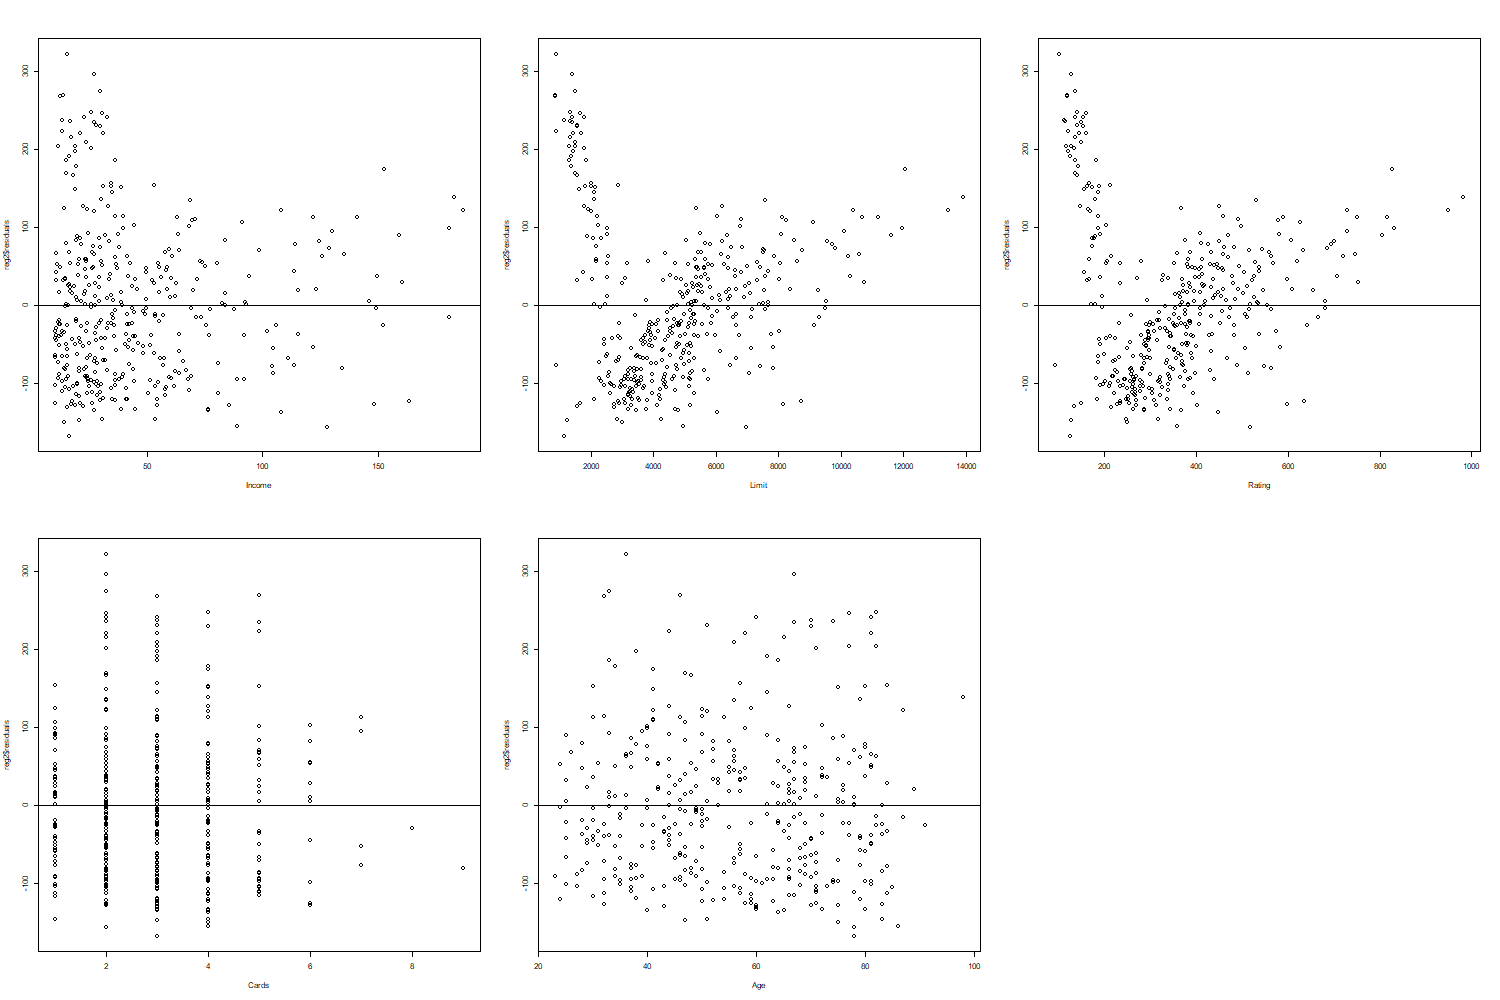
\includegraphics[scale=0.45]{Residual Plots}
\end{center}


% Model Selection
\begin{table}[H] \centering 
  \caption{Model Selection} 
  \label{} 
\resizebox{15.92cm}{!}{
\begin{tabular}{@{\extracolsep{5pt}}lccc} 
\\[-1.8ex]\hline 
\hline \\[-1.8ex] 
 & \multicolumn{3}{c}{\textit{Dependent variable:}} \\ 
\cline{2-4} 
\\[-1.8ex] & \multicolumn{3}{c}{Balance} \\ 
\\[-1.8ex] & (1) & (2) & (3)\\ 
\hline \\[-1.8ex] 
 Income & $-$7.816$^{***}$ & $-$6.283$^{***}$ & $-$6.238$^{***}$ \\ 
  & (0.235) & (0.488) & (0.486) \\ 
  & & & \\ 
 Limit & 0.189$^{***}$ &  &  \\ 
  & (0.033) &  &  \\ 
  & & & \\ 
 I(Income$\hat{\mkern6mu}$2) &  & $-$0.021$^{***}$ & $-$0.021$^{***}$ \\ 
  &  & (0.003) & (0.003) \\ 
  & & & \\ 
 Rating & 1.166$^{**}$ & 2.481$^{***}$ & 2.471$^{***}$ \\ 
  & (0.491) & (0.136) & (0.136) \\ 
  & & & \\ 
 I(Rating$\hat{\mkern6mu}$2) &  & 0.002$^{***}$ & 0.002$^{***}$ \\ 
  &  & (0.0002) & (0.0002) \\ 
  & & & \\ 
 Cards & 17.760$^{***}$ & 2.825 &  \\ 
  & (4.346) & (3.255) &  \\ 
  & & & \\ 
 Age & $-$0.598$^{**}$ & $-$0.714$^{***}$ & $-$0.729$^{***}$ \\ 
  & (0.295) & (0.263) & (0.261) \\ 
  & & & \\ 
 Edu\_BinsBachelors & 6.884 & 5.757 &  \\ 
  & (11.901) & (10.604) &  \\ 
  & & & \\ 
 Edu\_BinsPost-Grad & $-$5.565 & $-$9.563 &  \\ 
  & (12.329) & (11.000) &  \\ 
  & & & \\ 
 GenderFemale & $-$10.894 & $-$9.118 &  \\ 
  & (9.925) & (8.845) &  \\ 
  & & & \\ 
 StudentYes & 426.109$^{***}$ & 429.092$^{***}$ & 428.341$^{***}$ \\ 
  & (16.774) & (14.920) & (14.755) \\ 
  & & & \\ 
 MarriedYes & $-$8.535 & $-$12.380 &  \\ 
  & (10.361) & (9.195) &  \\ 
  & & & \\ 
 EthnicityAsian & 15.965 & 20.348 &  \\ 
  & (14.157) & (12.593) &  \\ 
  & & & \\ 
 EthnicityCaucasian & 10.027 & 13.903 &  \\ 
  & (12.217) & (10.902) &  \\ 
  & & & \\ 
 Constant & $-$497.360$^{***}$ & $-$339.084$^{***}$ & $-$329.576$^{***}$ \\ 
  & (29.040) & (30.994) & (26.542) \\ 
  & & & \\ 
\hline \\[-1.8ex] 
Observations & 400 & 400 & 400 \\ 
R$^{2}$ & 0.955 & 0.964 & 0.964 \\ 
Adjusted R$^{2}$ & 0.954 & 0.963 & 0.963 \\ 
Residual Std. Error & 98.853 (df = 387) & 88.081 (df = 386) & 88.218 (df = 393) \\ 
F Statistic & 686.991$^{***}$ (df = 12; 387) & 806.545$^{***}$ (df = 13; 386) & 1,740.723$^{***}$ (df = 6; 393) \\ 
\hline 
\hline \\[-1.8ex] 
\textit{Note:}  & \multicolumn{3}{r}{$^{*}$p$<$0.1; $^{**}$p$<$0.05; $^{***}$p$<$0.01} \\ 
\end{tabular} 
}
\end{table}


\section*{Bank's Marketing Success}
\subsection*{Question 2.1}
$$Pr(y_i = 1|duration_i) = \frac{\exp(\beta_0+\beta_1dist_i)}{1+\exp(\beta_0+\beta_1dist_i)}$$ 
$$Pr(y_i = 0|duration_i) = \frac{1}{1+\exp(\beta_0+\beta_1dist_i)}$$ 


\subsection*{Question 2.2}
$$\ell(\beta|\mathbf{y},\mathbf{X}) = \sum\limits_{i=1}^n \left[ y_i \ln{\left( \frac{\exp(\beta_0+\beta_1dist_i)}{1+\exp(\beta_0+\beta_1dist_i)}\right)} + (1-y_i) \ln{\left( \frac{1}{1+\exp(\beta_0+\beta_1dist_i)}\right)}\right]$$


}
\end{document}